\documentclass[aspectratio=169, 10pt]{beamer}

% --- THEME & FONTS (XELATEX VIETNAMESE SUPPORT) ---
\usetheme{Madrid}
\usepackage{fontspec}
\setmainfont{Arial}
\setsansfont{Arial}

% --- ESSENTIAL PACKAGES ---
\usepackage{amsmath, amssymb, amsfonts}
\usepackage{graphicx}
\usepackage{booktabs}
\usepackage{array}
\usepackage{tabularx}
\newcolumntype{Y}{>{\raggedright\arraybackslash}X}
\usepackage{hyperref}

% --- COLOR DEFINITIONS ---
\definecolor{primaryNavy}{RGB}{20, 45, 85}
\definecolor{accentTeal}{RGB}{13, 148, 136}
\definecolor{accentOrange}{RGB}{217, 95, 2}
\definecolor{bgSlate}{RGB}{248, 250, 252}
\definecolor{textDark}{RGB}{30, 41, 59}

\setbeamercolor{palette primary}{bg=primaryNavy, fg=white}
\setbeamercolor{palette secondary}{bg=accentTeal, fg=white}
\setbeamercolor{palette tertiary}{bg=primaryNavy!90, fg=white}
\setbeamercolor{title}{bg=primaryNavy, fg=white}
\setbeamercolor{frametitle}{bg=primaryNavy, fg=white}
\setbeamercolor{structure}{fg=primaryNavy}
\setbeamercolor{block title}{bg=primaryNavy, fg=white}
\setbeamercolor{block body}{bg=primaryNavy!8, fg=textDark}
\setbeamercolor{block title alerted}{bg=accentOrange, fg=white}
\setbeamercolor{block body alerted}{bg=accentOrange!10, fg=textDark}
\setbeamercolor{block title example}{bg=accentTeal, fg=white}
\setbeamercolor{block body example}{bg=accentTeal!10, fg=textDark}

% Remove navigation symbols
\setbeamertemplate{navigation symbols}{}

% Custom footer
\setbeamertemplate{footline}{
  \leavevmode%
  \hbox{%
  \begin{beamercolorbox}[wd=.5\paperwidth,ht=2.25ex,dp=1ex,left]{title in head/foot}%
    \hspace*{2ex}\usebeamerfont{title in head/foot}Khám Phá Dữ Liệu \& Kiểm Toán Chất Lượng (EDA \& Data Quality)
  \end{beamercolorbox}%
  \begin{beamercolorbox}[wd=.5\paperwidth,ht=2.25ex,dp=1ex,right]{date in head/foot}%
    \usebeamerfont{date in head/foot}\insertframenumber{} / \inserttotalframenumber\hspace*{2ex}
  \end{beamercolorbox}}%
  \vskip0pt%
}

% --- METADATA ---
\title[EDA \& Data Quality]{\textbf{Khám Phá Dữ Liệu \& Kiểm Toán Chất Lượng}}
\author{}
\institute{}
\date{}

\begin{document}

% ==============================================================================
% SLIDE 1: TIÊU ĐỀ
% ==============================================================================
\begin{frame}[plain]
  \vfill
  \centering
  \begin{beamercolorbox}[sep=14pt,center,rounded=true,shadow=true]{title}
    {\usebeamerfont{title}\textbf{\Large Khám Phá Dữ Liệu (EDA) \& Kiểm Toán Chất Lượng Dữ Liệu}}\\[0.25cm]
    {\normalsize\textsf{Nền Tảng Thực Nghiệm Cho Bài Toán Dự Đoán Xác Suất Mua Hàng Bán Lẻ}}
  \end{beamercolorbox}
  \vfill
\end{frame}
\addtocounter{framenumber}{-1}

% ==============================================================================
% SLIDE 2: BỐI CẢNH & MỤC TIÊU EDA
% ==============================================================================
\begin{frame}{1. Bối Cảnh Thực Nghiệm \& Mục Tiêu Khám Phá Dữ Liệu}
  \begin{columns}[T]
    \begin{column}{0.48\textwidth}
      \textbf{Thách Thức Dữ Liệu Bán Lẻ Gốc:}
      \begin{itemize}\setlength{\itemsep}{4pt}
        \item \textbf{Quy mô lớn \& phức tạp:} 2.6 triệu giao dịch từ 2,500 hộ gia đình trong 711 ngày liên tục.
        \item \textbf{Nhiễu dữ liệu nghiệp vụ:} Lỗi hủy quét POS, hàng tặng 0đ, độ phủ nhân khẩu học không đồng đều.
        \item \textbf{Kỷ luật thời gian:} Thiết lập ranh giới quá khứ ($DAY \le t_0$) và tương lai ($DAY > t_0$).
      \end{itemize}
    \end{column}
    
    \begin{column}{0.48\textwidth}
      \begin{alertblock}{Mục Tiêu Kiểm Toán Chất Lượng}
        Lọc 942 giỏ dị biệt, khử trùng 5,164 dòng coupon, xử lý khuyết thiếu nhân khẩu, bảo toàn 100\% tập mẫu.
      \end{alertblock}
      \vspace{0.2cm}
      \begin{exampleblock}{Mục Tiêu Khám Phá Nghiệp Vụ \& Hành Vi}
        Chiết xuất \textbf{15 phát hiện thực nghiệm cốt lõi} (10 quy luật hành vi ML + 5 góc nhìn chiến lược bán lẻ \& CRM) nhằm xác định cửa sổ dự báo tối ưu ($\Delta t$) và định hình chiến lược tăng trưởng doanh thu.
      \end{exampleblock}
    \end{column}
  \end{columns}
\end{frame}

% ==============================================================================
% SLIDE 3: KIẾN TRÚC 8 BẢNG DỮ LIỆU & KẾT QUẢ KIỂM TOÁN LÀM SẠCH
% ==============================================================================
\begin{frame}{2. Kiến Trúc 8 Bảng Dữ Liệu \& Kiểm Toán Chất Lượng}
  \centering
  \footnotesize
  \setlength{\tabcolsep}{5pt}
  \renewcommand{\arraystretch}{1.12}
  \begin{tabularx}{\textwidth}{llrrY}
    \toprule
    \textbf{Bảng Dữ Liệu} & \textbf{Khóa Chính / Liên Kết} & \textbf{Số Dòng} & \textbf{Độ Phủ} & \textbf{Vai Trò Nghiệp Vụ \& Kiểm Toán Chất Lượng} \\
    \midrule
    \texttt{transactions} & Dòng hóa đơn & 2,595,732 & 2,500 hộ & Lịch sử 711 ngày; loại 942 giỏ $\le \$0$, bảo toàn đúng 275,542 giỏ hàng thương mại thuần túy \\
    \texttt{products} & Mã sản phẩm & 92,353 & 44 ngành & Phân loại danh mục hàng hóa, bóc tách thực phẩm tươi sống \\
    \texttt{demographics} & Mã hộ gia đình & 801 & 32.0\% & Tuổi, thu nhập, quy mô; xử lý \texttt{UNKNOWN} cho 68\% hộ thiếu dữ liệu \\
    \texttt{campaign\_desc} & Mã chiến dịch & 30 & Toàn bộ & Lịch trình hoạt động tiếp thị (phân loại chiến dịch A, B, C) \\
    \texttt{campaigns} & Hộ + Chiến dịch & 7,208 & 1,584 hộ & Danh sách hộ gia đình được gửi thư ưu đãi tiếp thị tận nhà \\
    \texttt{coupons} & Mã ưu đãi + SKU & 124,548 & Toàn bộ & Ánh xạ SKU; khử trùng \textbf{5,164 bản ghi trùng} (còn 119,384 dòng) \\
    \texttt{redemptions} & Lượt đổi phiếu & 2,318 & 434 hộ & Lịch sử dùng coupon tại quầy; kiểm toán đạt 0 dòng trùng lặp \\
    \texttt{causal\_data} & Tuần + Cửa hàng & 36,786,524 & Toàn bộ & Vị trí trưng bày quầy kệ nổi bật \& tờ rơi khuyến mãi phát hành \\
    \bottomrule
  \end{tabularx}
\end{frame}

% ==============================================================================
% SLIDE 4: CÂU CHUYỆN 1 - NHỊP SINH HỌC ĐI CHỢ
% ==============================================================================
\begin{frame}{3. Nhịp Sinh Học Đi Chợ \& Chu Kỳ Mua Sắm Của Hộ Gia Đình}
  \begin{columns}[c]
    \begin{column}{0.60\textwidth}
      \centering
      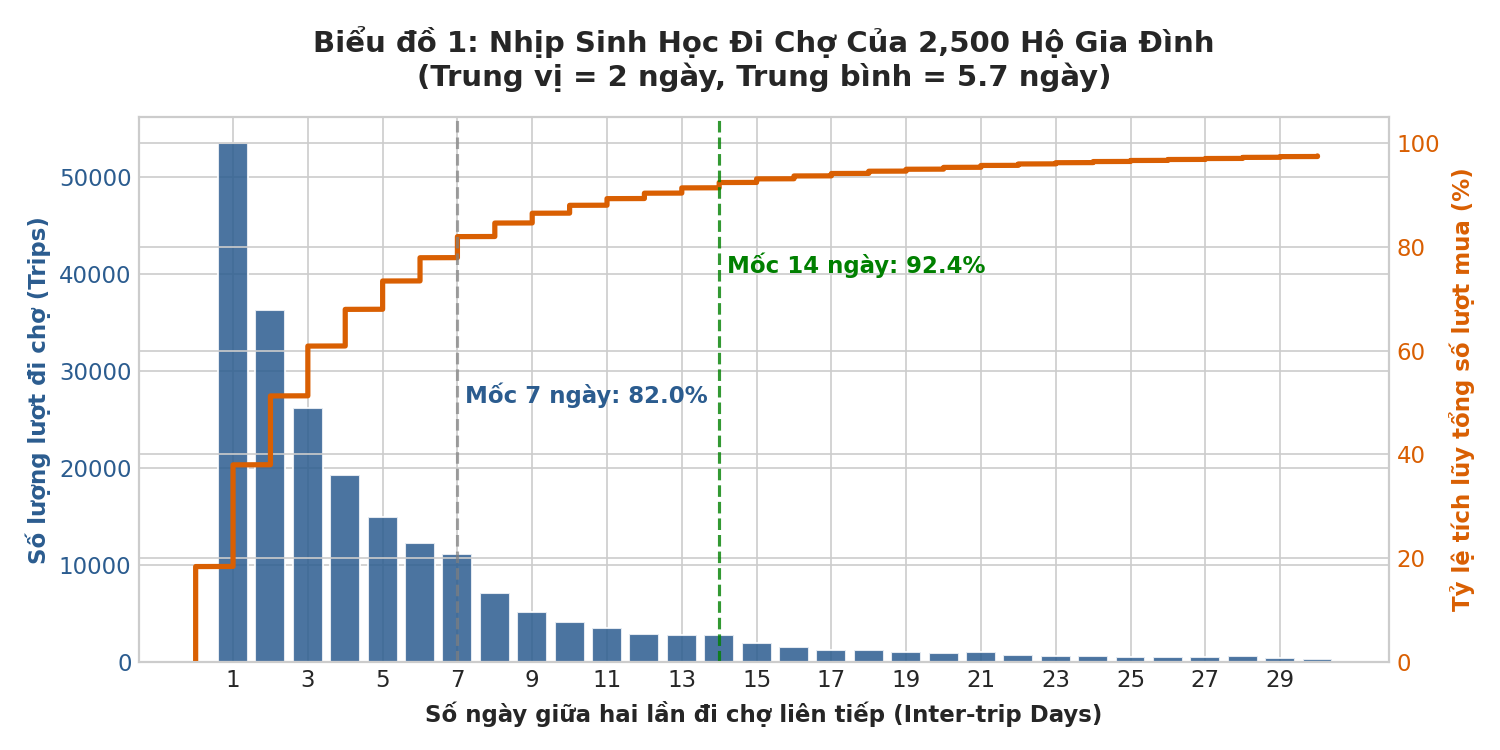
\includegraphics[width=\linewidth,height=0.65\textheight,keepaspectratio]{../reports/figures/01_inter_trip_distribution.png}
    \end{column}
    \begin{column}{0.38\textwidth}
      \small
      \textbf{Quy Luật Hành Vi Đi Chợ:}
      \begin{itemize}\setlength{\itemsep}{2pt}
        \item \textbf{Tần suất thiết yếu:} Khách đi chợ theo nhịp tuần; hơn 80\% lượt mua lặp lại trong $\le 7$ ngày.
        \item \textbf{Bão hòa chu kỳ:} Đạt 92.4\% ở mốc 14 ngày; thời gian chờ lâu hơn là khách vãng lai.
      \end{itemize}
      \vspace{0.08cm}
      \begin{alertblock}{Cơ Sở Chọn $\Delta t = 14$ Ngày}
        \footnotesize
        Bao quát trọn \textbf{92.4\% hành vi tự nhiên}, tạo cửa sổ hành động lý tưởng cho CRM.\\
        $\rightarrow$ Biến: \texttt{urgency\_ratio}, \texttt{days\_since\_last\_basket}.
      \end{alertblock}
    \end{column}
  \end{columns}
\end{frame}

% ==============================================================================
% SLIDE 5: CÂU CHUYỆN 2 - CẤU TRÚC GIÁ TRỊ GIỎ HÀNG
% ==============================================================================
\begin{frame}{4. Cấu Trúc Giá Trị Giỏ Hàng Thực Nghiệm (AOV)}
  \begin{columns}[c]
    \begin{column}{0.60\textwidth}
      \centering
      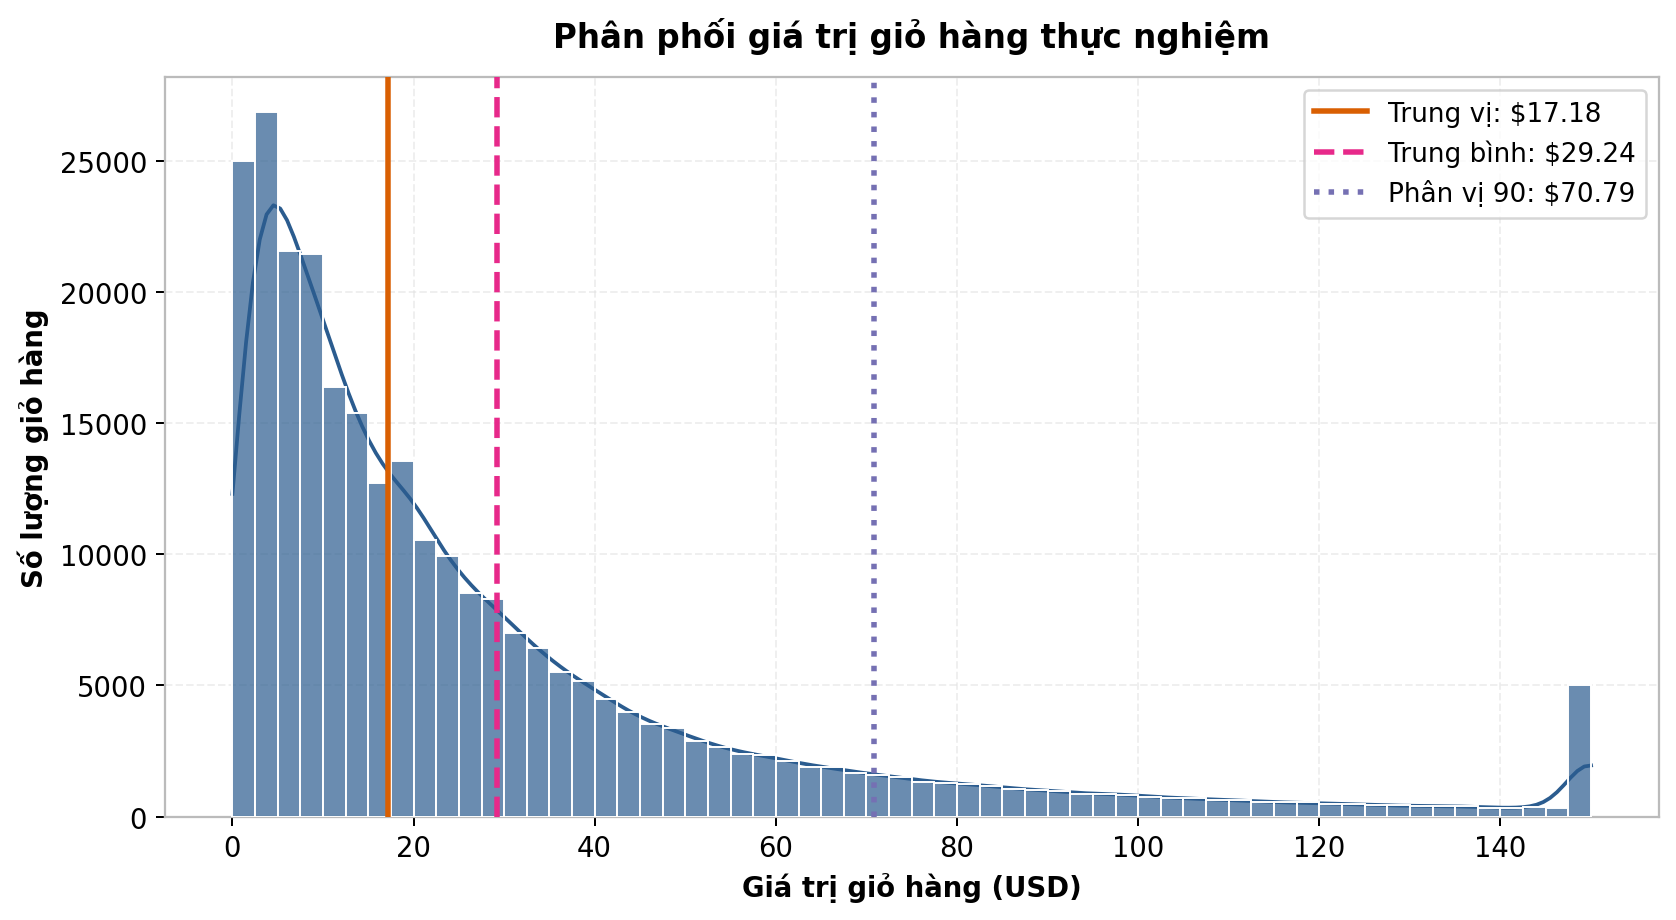
\includegraphics[width=\linewidth,height=0.65\textheight,keepaspectratio]{../reports/figures/02_basket_spend_distribution.png}
    \end{column}
    \begin{column}{0.38\textwidth}
      \small
      \textbf{Đặc Trưng Phân Hóa Giỏ Hàng:}
      \begin{itemize}\setlength{\itemsep}{2pt}
        \item \textbf{Lệch phải điển hình:} Đa số đơn hàng là mua sắm lẻ bổ sung, nhưng nhóm giỏ lớn gánh doanh số.
        \item \textbf{Nhiễu số trung bình:} AOV cao hơn P50 tới 70\% do ảnh hưởng của các đơn mua sỉ/tiệc tùng.
      \end{itemize}
      \vspace{0.08cm}
      \begin{exampleblock}{Quyết Định Kỹ Thuật}
        \footnotesize
        Khách mua nhiều tiền chưa chắc đã đi thường xuyên; bắt buộc bóc tách:\\
        $\rightarrow$ \textbf{Tần suất} (\texttt{frequency}) \& \textbf{Giá trị} (\texttt{spend\_30d}, \texttt{aov\_90d}).
      \end{exampleblock}
    \end{column}
  \end{columns}
\end{frame}

% ==============================================================================
% SLIDE 5: CÂU CHUYỆN 3 - ĐỒ TƯƠI SỐNG
% ==============================================================================
\begin{frame}{5. Thực Phẩm Tươi Sống \& Động Lực Thúc Đẩy Mua Sắm}
  \begin{columns}[c]
    \begin{column}{0.60\textwidth}
      \centering
      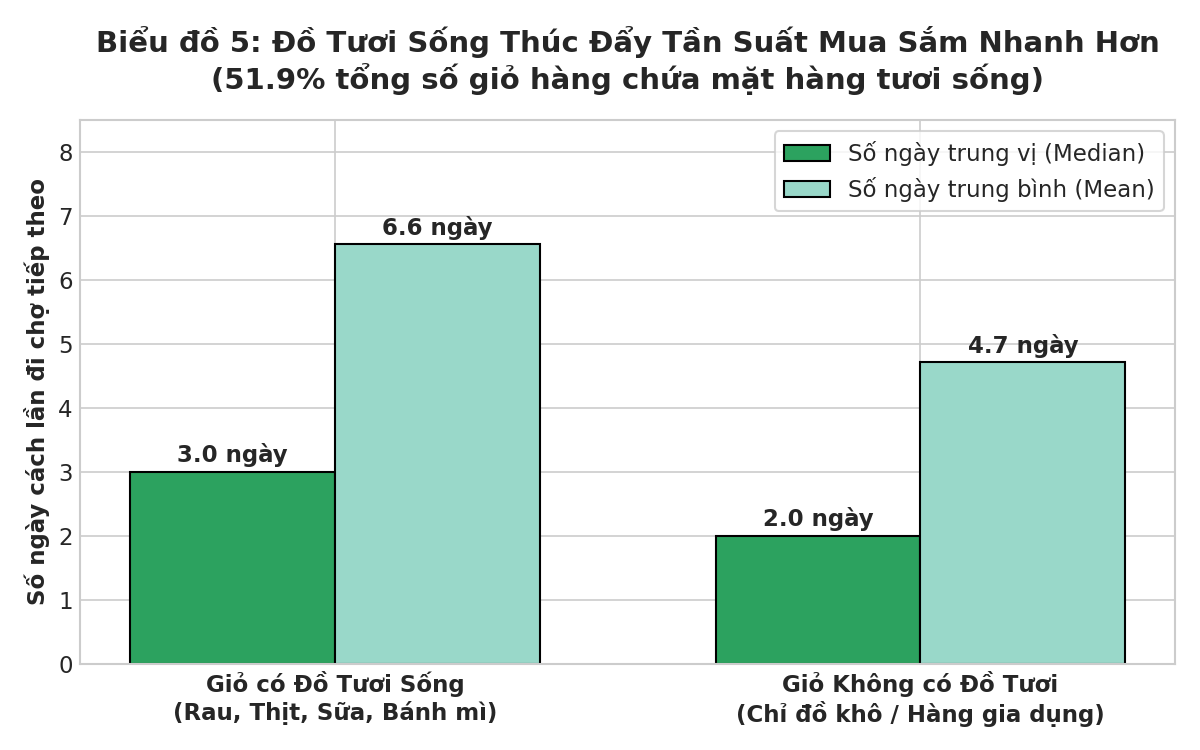
\includegraphics[width=\linewidth,height=0.65\textheight,keepaspectratio]{../reports/figures/05_perishable_trigger_effect.png}
    \end{column}
    \begin{column}{0.38\textwidth}
      \small
      \textbf{Cơ Chế Tiêu Dùng Tươi Sống:}
      \begin{itemize}\setlength{\itemsep}{2pt}
        \item \textbf{Đồng hồ đếm ngược:} Hạn dùng ngắn (2--5 ngày) của thịt, rau, sữa buộc hộ phải đi chợ lại sớm.
        \item \textbf{Rút ngắn độ trễ:} Mua đồ tươi kéo thời gian chờ tái mua giảm gần 2 ngày so với chỉ mua đồ khô.
      \end{itemize}
      \vspace{0.08cm}
      \begin{exampleblock}{Đặc Trưng Cốt Lõi}
        \footnotesize
        Cạn thực phẩm tủ lạnh kích thích chuyến đi kế tiếp.\\
        $\rightarrow$ Biến: \texttt{days\_since\_last\_perishable}, \texttt{perishable\_ratio\_90d}.
      \end{exampleblock}
    \end{column}
  \end{columns}
\end{frame}

% ==============================================================================
% SLIDE 6: CÂU CHUYỆN 4 - MỎ NEO ĐA NGÀNH
% ==============================================================================
\begin{frame}{6. Độ Phủ Ngành Hàng \& Hiệu Ứng Mỏ Neo Giữ Chân Khách Hàng}
  \begin{columns}[c]
    \begin{column}{0.60\textwidth}
      \centering
      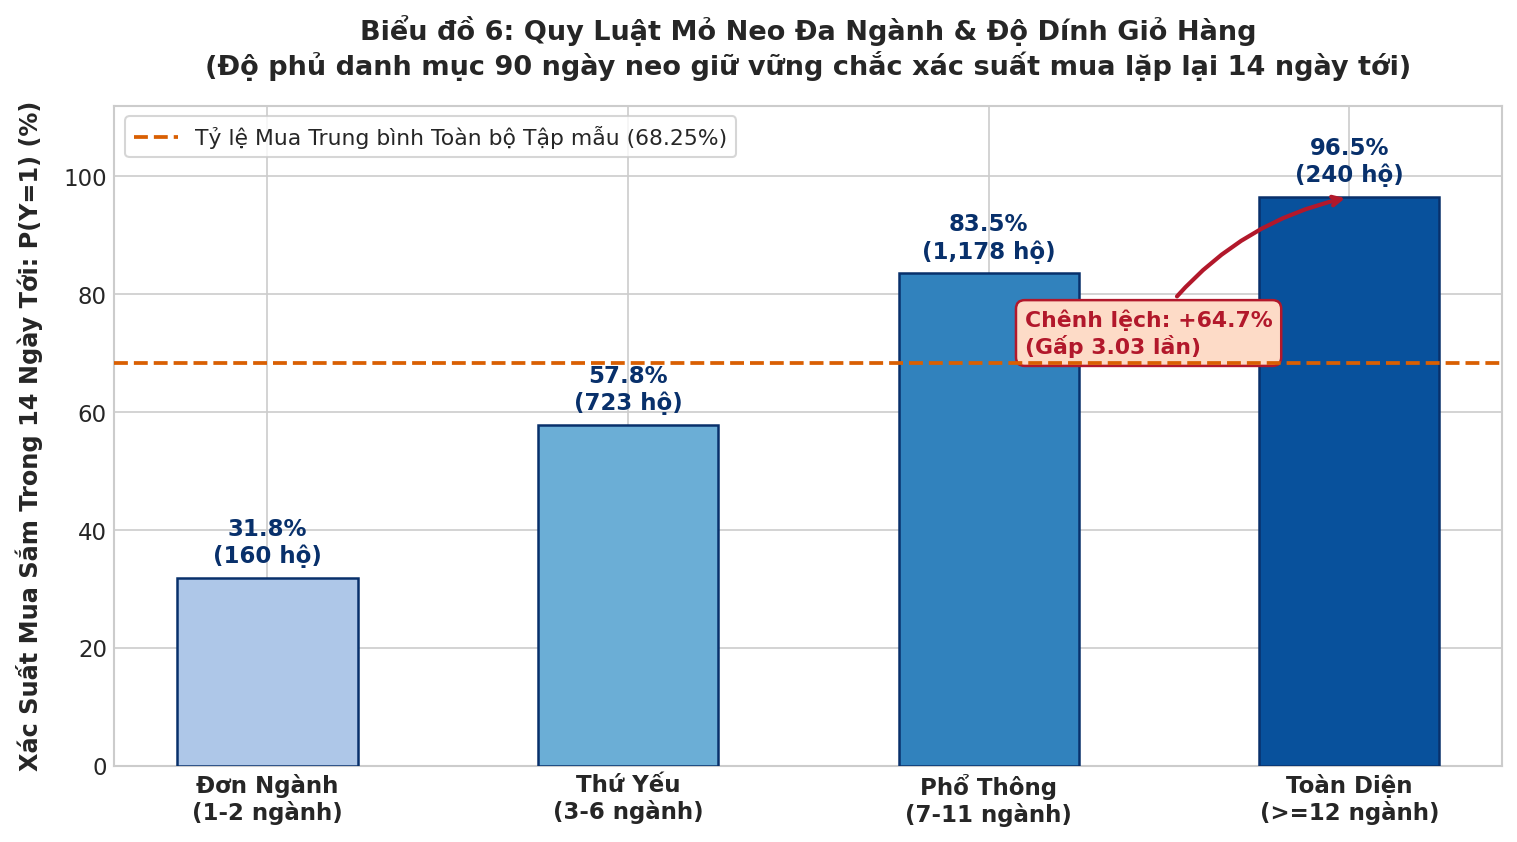
\includegraphics[width=\linewidth,height=0.65\textheight,keepaspectratio]{../reports/figures/24_category_breadth_stickiness.png}
    \end{column}
    \begin{column}{0.38\textwidth}
      \small
      \textbf{Quy Luật Mỏ Neo Đa Ngành:}
      \begin{itemize}\setlength{\itemsep}{2pt}
        \item \textbf{Phân hóa cực độ (+64.7\%):} Hộ mua $\ge 12$ ngành có xác suất mua tới \textbf{96.5\%}; hộ chỉ mua 1--2 ngành rơi về \textbf{31.8\%}.
        \item \textbf{Khách toàn diện vs Vãng lai:} Giỏ hàng đa ngành biến siêu thị thành điểm đến thiết yếu toàn diện (One-Stop Destination).
      \end{itemize}
      \vspace{0.08cm}
      \begin{alertblock}{Đặc Trưng Dự Báo Then Chốt}
        \footnotesize
        Độ rộng giỏ hàng là mỏ neo giữ chân khách hàng mạnh nhất:\\
        $\rightarrow$ Biến: \texttt{department\_breadth\_90d}, \texttt{avg\_items\_per\_basket\_90d}.
      \end{alertblock}
    \end{column}
  \end{columns}
\end{frame}

% ==============================================================================
% SLIDE 7: CÂU CHUYỆN 5 - HIỆU ỨNG MỒI CÂU COUPON
% ==============================================================================
\begin{frame}{7. Hiệu Ứng Mồi Câu \& Độ Lan Tỏa Của Phiếu Giảm Giá}
  \begin{columns}[c]
    \begin{column}{0.60\textwidth}
      \centering
      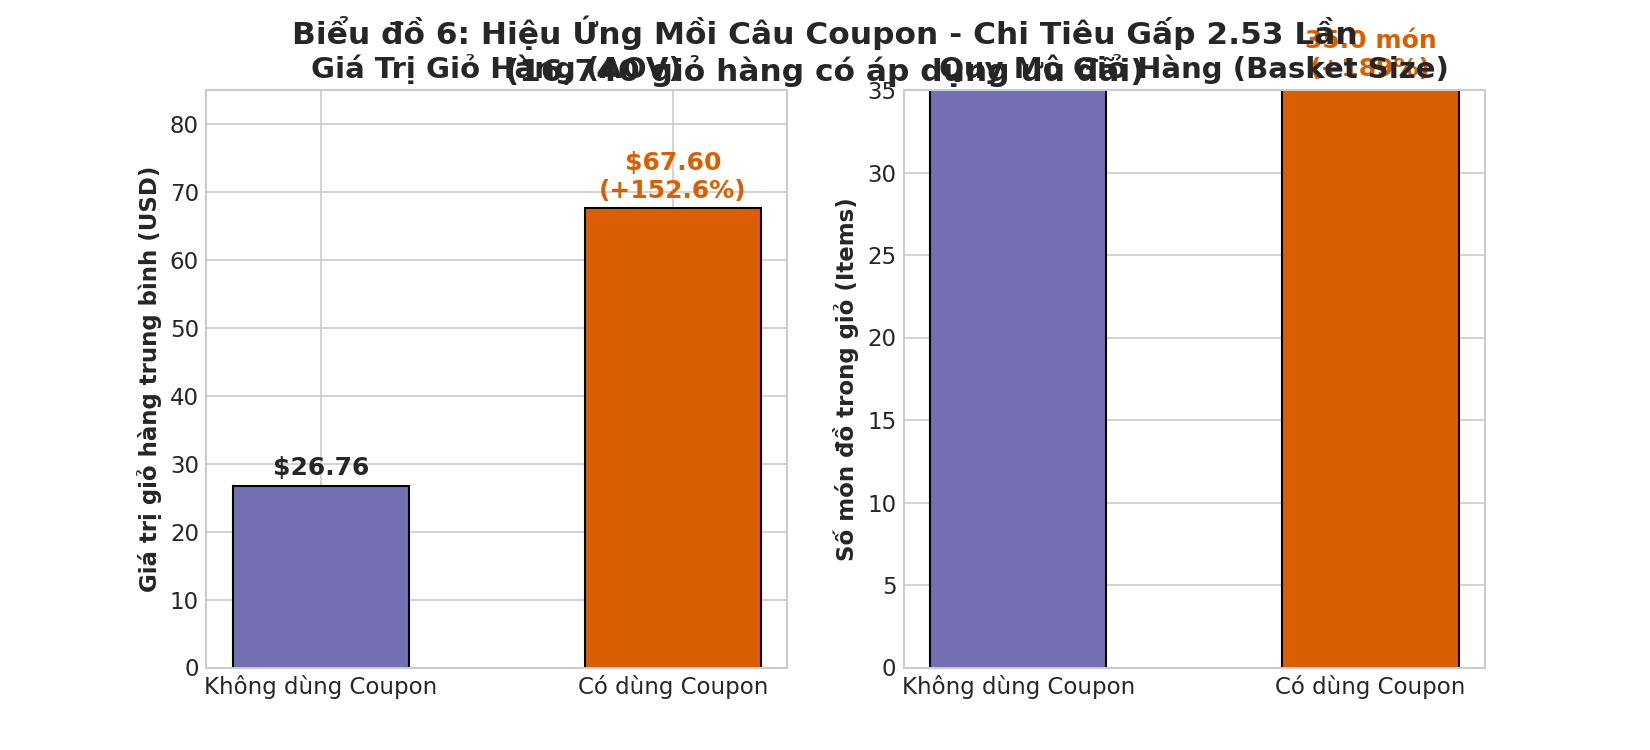
\includegraphics[width=\linewidth,height=0.65\textheight,keepaspectratio]{../reports/figures/06_coupon_halo_effect.png}
    \end{column}
    \begin{column}{0.38\textwidth}
      \small
      \textbf{Cơ Chế Lan Tỏa (Halo Effect):}
      \begin{itemize}\setlength{\itemsep}{2pt}
        \item \textbf{Tâm lý mồi câu:} Phiếu giảm giá chỉ nhắm 1--2 món, nhưng kéo khách dạo khắp các quầy khác.
        \item \textbf{Chi tiêu chéo nguyên giá:} Hơn 80\% giá trị giỏ hàng đến từ các sản phẩm nguyên giá đi kèm.
      \end{itemize}
      \vspace{0.08cm}
      \begin{alertblock}{Bản Chất Kinh Doanh}
        \footnotesize
        Hộ chịu dùng coupon là nhóm khách có giá trị cao nhất.\\
        $\rightarrow$ Biến: \texttt{coupon\_redempt\_count\_180d}.
      \end{alertblock}
    \end{column}
  \end{columns}
\end{frame}

% ==============================================================================
% SLIDE 8: CÂU CHUYỆN 6 - GIA TỐC CHIẾN DỊCH TIẾP THỊ
% ==============================================================================
\begin{frame}{8. Sức Bật Chu Kỳ Từ Các Chiến Dịch Tiếp Thị}
  \begin{columns}[c]
    \begin{column}{0.60\textwidth}
      \centering
      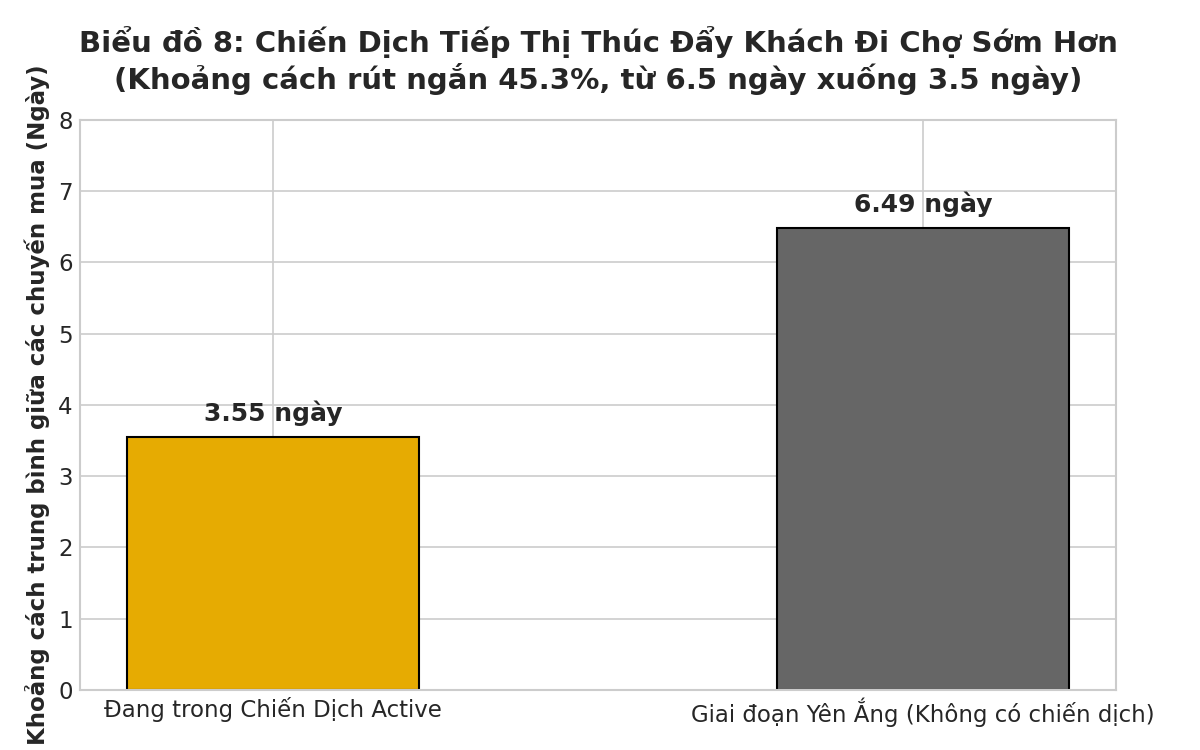
\includegraphics[width=\linewidth,height=0.65\textheight,keepaspectratio]{../reports/figures/07_campaign_acceleration.png}
    \end{column}
    \begin{column}{0.38\textwidth}
      \small
      \textbf{Tác Động Xung Lực Tiếp Thị:}
      \begin{itemize}\setlength{\itemsep}{2pt}
        \item \textbf{Phá vỡ độ ì mua sắm:} Thư tiếp thị gửi tận nhà kích thích nhu cầu tiềm ẩn, kéo khách quay lại sớm gần 3 ngày.
        \item \textbf{Tăng mật độ giao dịch:} Trong đợt chiến dịch active, tần suất mua sắm tăng vọt gần gấp đôi.
      \end{itemize}
      \vspace{0.08cm}
      \begin{block}{Quyết Định Kỹ Thuật}
        \footnotesize
        Chiến dịch là chất xúc tác ngoại sinh tăng tốc chu kỳ.\\
        $\rightarrow$ Biến: \texttt{is\_targeted\_by\_active\_campaign}.
      \end{block}
    \end{column}
  \end{columns}
\end{frame}

% ==============================================================================
% SLIDE 9: CÂU CHUYỆN 7 - HIỆN TƯỢNG NHẢY CÓC CỬA HÀNG
% ==============================================================================
\begin{frame}{9. Hành Vi Mua Sắm Đa Cửa Hàng \& Lòng Trung Thành}
  \begin{columns}[c]
    \begin{column}{0.60\textwidth}
      \centering
      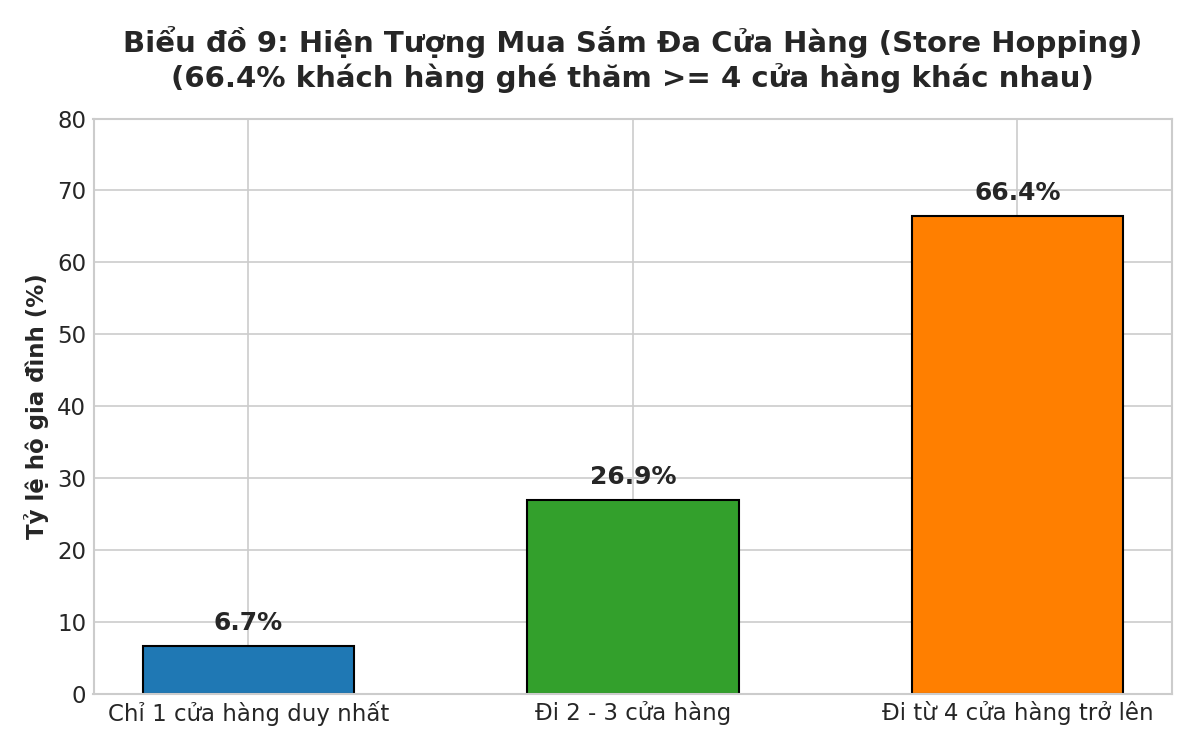
\includegraphics[width=\linewidth,height=0.65\textheight,keepaspectratio]{../reports/figures/08_store_hopping_distribution.png}
    \end{column}
    \begin{column}{0.38\textwidth}
      \small
      \textbf{Quy Luật Phân Bổ Địa Bàn:}
      \begin{itemize}\setlength{\itemsep}{2pt}
        \item \textbf{Linh hoạt điểm đến:} Khách mua chéo nhiều chi nhánh tiện đường đi làm, đón con hoặc du lịch.
        \item \textbf{Tập trung ngân sách lõi:} Dù ghé nhiều nơi, gần 3/4 ngân sách vẫn đổ vào một cửa hàng ruột duy nhất.
      \end{itemize}
      \vspace{0.08cm}
      \begin{exampleblock}{Quyết Định Kỹ Thuật}
        \footnotesize
        Cần phân định chi nhánh vãng lai với chi nhánh trọng tâm:\\
        $\rightarrow$ Biến: \texttt{store\_loyalty\_index}, \texttt{primary\_store\_id}.
      \end{exampleblock}
    \end{column}
  \end{columns}
\end{frame}

% ==============================================================================
% SLIDE 10: CÂU CHUYỆN 8 - NHÂN KHẨU HỌC & AOV
% ==============================================================================
\begin{frame}{10. Quy Mô Hộ Gia Đình \& Tác Động Lên Giá Trị Giỏ Hàng}
  \begin{columns}[c]
    \begin{column}{0.60\textwidth}
      \centering
      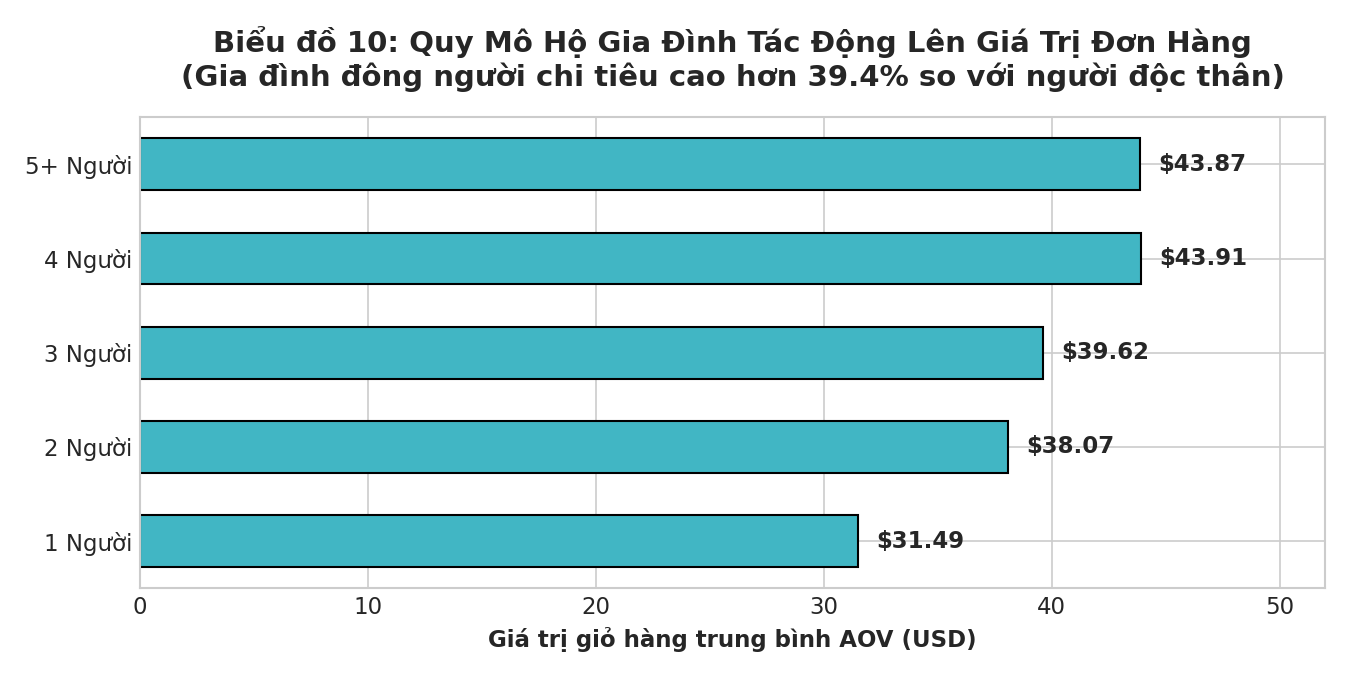
\includegraphics[width=\linewidth,height=0.65\textheight,keepaspectratio]{../reports/figures/09_household_size_vs_aov.png}
    \end{column}
    \begin{column}{0.38\textwidth}
      \small
      \textbf{Động Lực Nhân Khẩu Học:}
      \begin{itemize}\setlength{\itemsep}{2pt}
        \item \textbf{Tuyến tính theo quy mô:} Số miệng ăn trong nhà quy định trực tiếp kích thước hóa đơn thanh toán.
        \item \textbf{Hiệu ứng con cái:} Trẻ nhỏ bổ sung các nhóm hàng giá trị cao như sữa bột, tã bỉm và đồ ăn dặm.
      \end{itemize}
      \vspace{0.08cm}
      \begin{block}{Quyết Định Kỹ Thuật}
        \footnotesize
        Khai thác tín hiệu nhân khẩu qua phân loại khuyết thiếu:\\
        $\rightarrow$ Biến: \texttt{hh\_size}, \texttt{kid\_category}, \texttt{income\_group}.
      \end{block}
    \end{column}
  \end{columns}
\end{frame}

% ==============================================================================
% SLIDE 11: CÂU CHUYỆN 9 - ĐỘ ỔN ĐỊNH NHÃN MỤC TIÊU
% ==============================================================================
\begin{frame}{11. Độ Ổn Định Nhãn Mục Tiêu Theo Dòng Thời Gian}
  \begin{columns}[c]
    \begin{column}{0.60\textwidth}
      \centering
      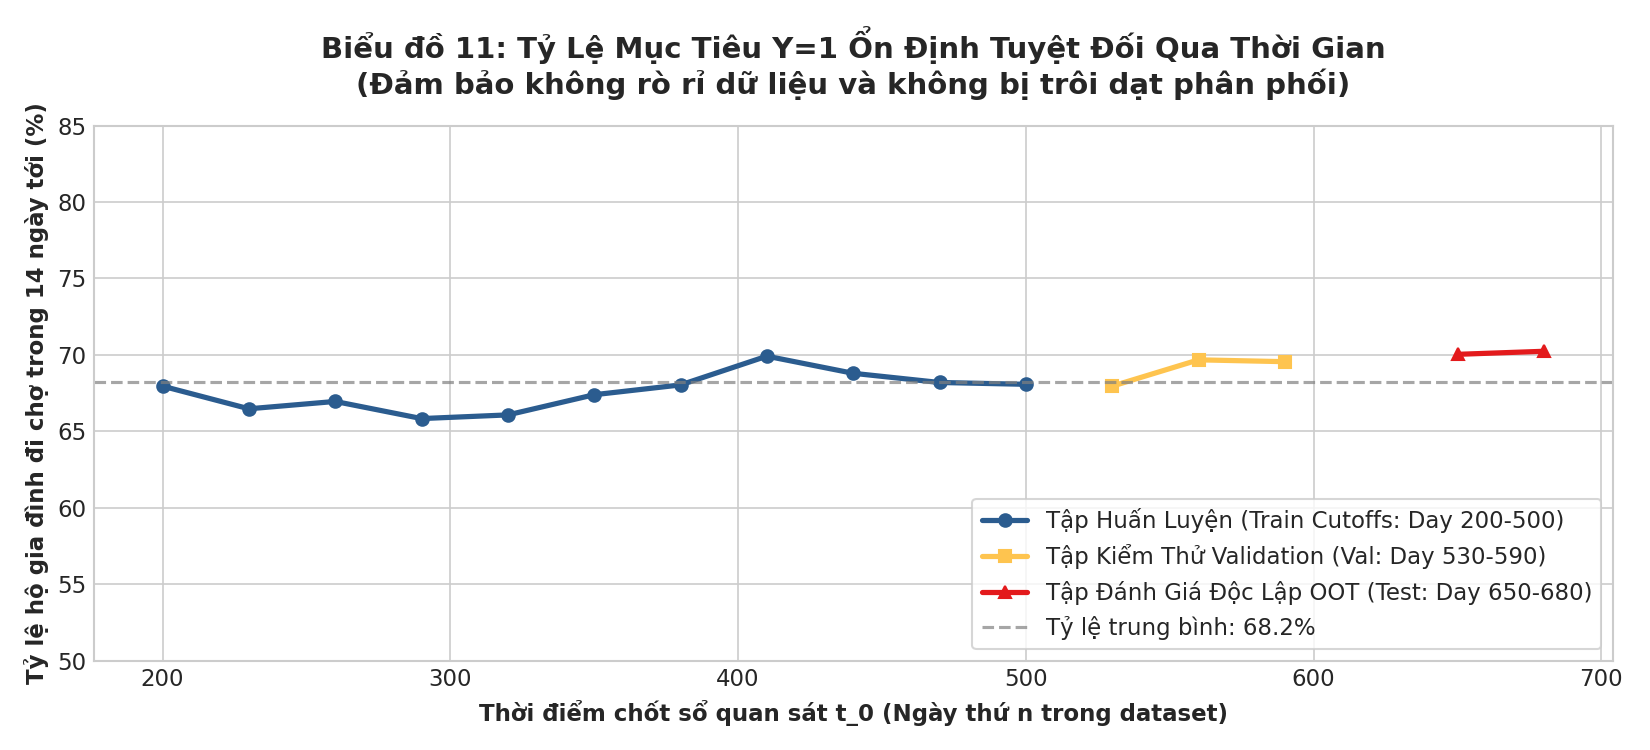
\includegraphics[width=\linewidth,height=0.65\textheight,keepaspectratio]{../reports/figures/10_target_rate_stability.png}
    \end{column}
    \begin{column}{0.38\textwidth}
      \small
      \textbf{Kiểm Định Tính Toàn Vẹn:}
      \begin{itemize}\setlength{\itemsep}{2pt}
        \item \textbf{Không trôi dạt dữ liệu:} Tỷ lệ đi chợ trong 14 ngày tới duy trì nhất quán quanh mức 68\% suốt 1.5 năm.
        \item \textbf{Biên dao động rất hẹp:} Chỉ $\pm 2.2\%$ khẳng định tính độc lập mùa vụ của nhịp bán lẻ thiết yếu.
      \end{itemize}
      \vspace{0.08cm}
      \begin{alertblock}{Kết Luận Kiểm Định}
        \footnotesize
        Nhãn ổn định tuyệt đối; vững chắc cho chiến lược Multi-cutoff trượt thời gian mà không méo mó phân phối.
      \end{alertblock}
    \end{column}
  \end{columns}
\end{frame}

% ==============================================================================
% SLIDE 12: CÂU CHUYỆN 10 - PHỄU CHUYỂN ĐỔI THEO LOẠI CHIẾN DỊCH
% ==============================================================================
\begin{frame}{12. Phễu Chuyển Đổi Tiếp Thị Theo Nhóm Chiến Dịch}
  \begin{columns}[c]
    \begin{column}{0.60\textwidth}
      \centering
      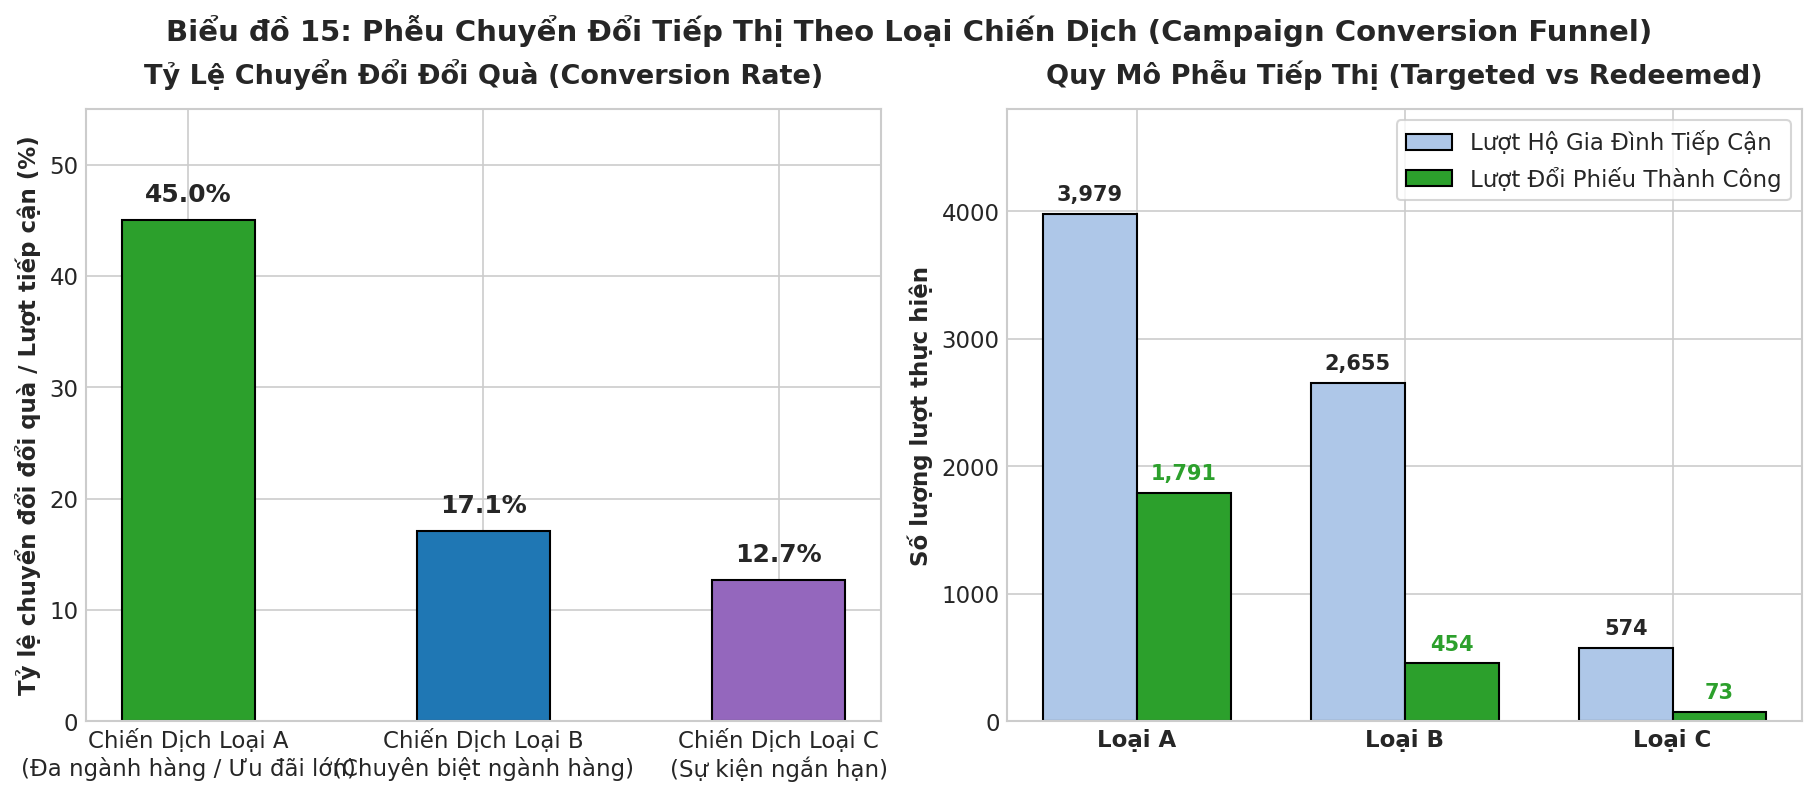
\includegraphics[width=\linewidth,height=0.65\textheight,keepaspectratio]{../reports/figures/22_campaign_type_conversion_funnel.png}
    \end{column}
    \begin{column}{0.38\textwidth}
      \small
      \textbf{Chiến Lược Tiếp Thị Đa Tầng:}
      \begin{itemize}\setlength{\itemsep}{1pt}
        \item \textbf{Ưu thế đa ngành (Loại A):} Độ phủ rộng giúp khách dễ tìm thấy ưu đãi phù hợp, tạo tỷ lệ đổi vượt trội.
        \item \textbf{Rào cản chuyên ngành (B \& C):} Ngành hẹp hoặc thời gian gấp rút giới hạn tỷ lệ chuyển đổi.
        \item \textbf{Phân hóa chất lượng:} Không phải chiến dịch nào cũng đem lại tác động thúc đẩy tương đương.
      \end{itemize}
      \vspace{0.06cm}
      \begin{alertblock}{Quyết Định Tiếp Thị \& ML}
        \footnotesize
        Mô hình bắt buộc phân rã theo loại hình chiến dịch:\\
        $\rightarrow$ Tách riêng: \texttt{is\_targeted\_by\_active\_campaign}.
      \end{alertblock}
    \end{column}
  \end{columns}
\end{frame}

% ==============================================================================
% SLIDE 14: CÂU CHUYỆN 13 - PHÂN HÓA CLV & PARETO
% ==============================================================================
\begin{frame}{13. Phân Hóa Giá Trị Trọn Đời (CLV) \& Kiểm Định Pareto 80/20}
  \begin{columns}[c]
    \begin{column}{0.60\textwidth}
      \centering
      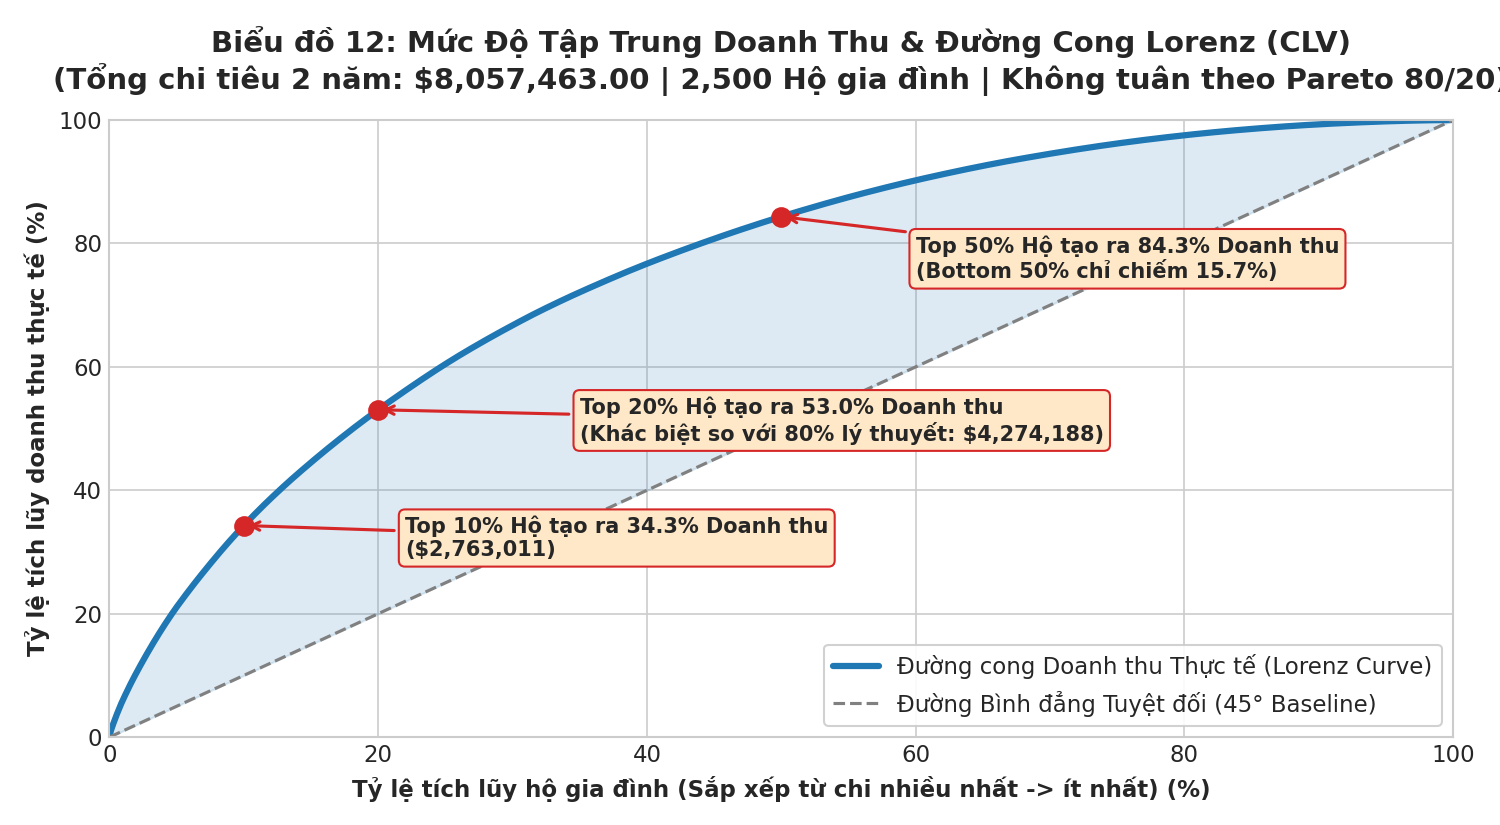
\includegraphics[width=\linewidth,height=0.65\textheight,keepaspectratio]{../reports/figures/19_clv_pareto_distribution.png}
    \end{column}
    \begin{column}{0.38\textwidth}
      \small
      \textbf{Kiểm Định Tập Trung Doanh Số:}
      \begin{itemize}\setlength{\itemsep}{2pt}
        \item \textbf{Độ dốc Lorenz:} Top 10\% hộ gánh 34.3\% doanh thu (\$2.76M); Top 20\% gánh 53.0\% (\$4.27M).
        \item \textbf{Bác bỏ Pareto 80/20 cực đoan:} Cần 44\% hộ để đạt 80\% doanh số; tiêu dùng thực phẩm thiết yếu phân bổ đều hơn hàng xa xỉ.
      \end{itemize}
      \vspace{0.08cm}
      \begin{alertblock}{Ứng Dụng CRM \& Handoff ML}
        \footnotesize
        Thiết lập phân khúc VIP bảo vệ dòng tiền; đặc trưng ML sử dụng \texttt{spend\_180d} quá khứ làm proxy an toàn, triệt tiêu rò rỉ CLV tương lai.
      \end{alertblock}
    \end{column}
  \end{columns}
\end{frame}

% ==============================================================================
% SLIDE 15: CÂU CHUYỆN 14 - CẤU TRÚC CHIẾT KHẤU 2 TẦNG
% ==============================================================================
\begin{frame}{14. Cấu Trúc Khuyến Mãi 2 Tầng: Niêm Yết vs Phiếu Giảm Giá}
  \begin{columns}[c]
    \begin{column}{0.60\textwidth}
      \centering
      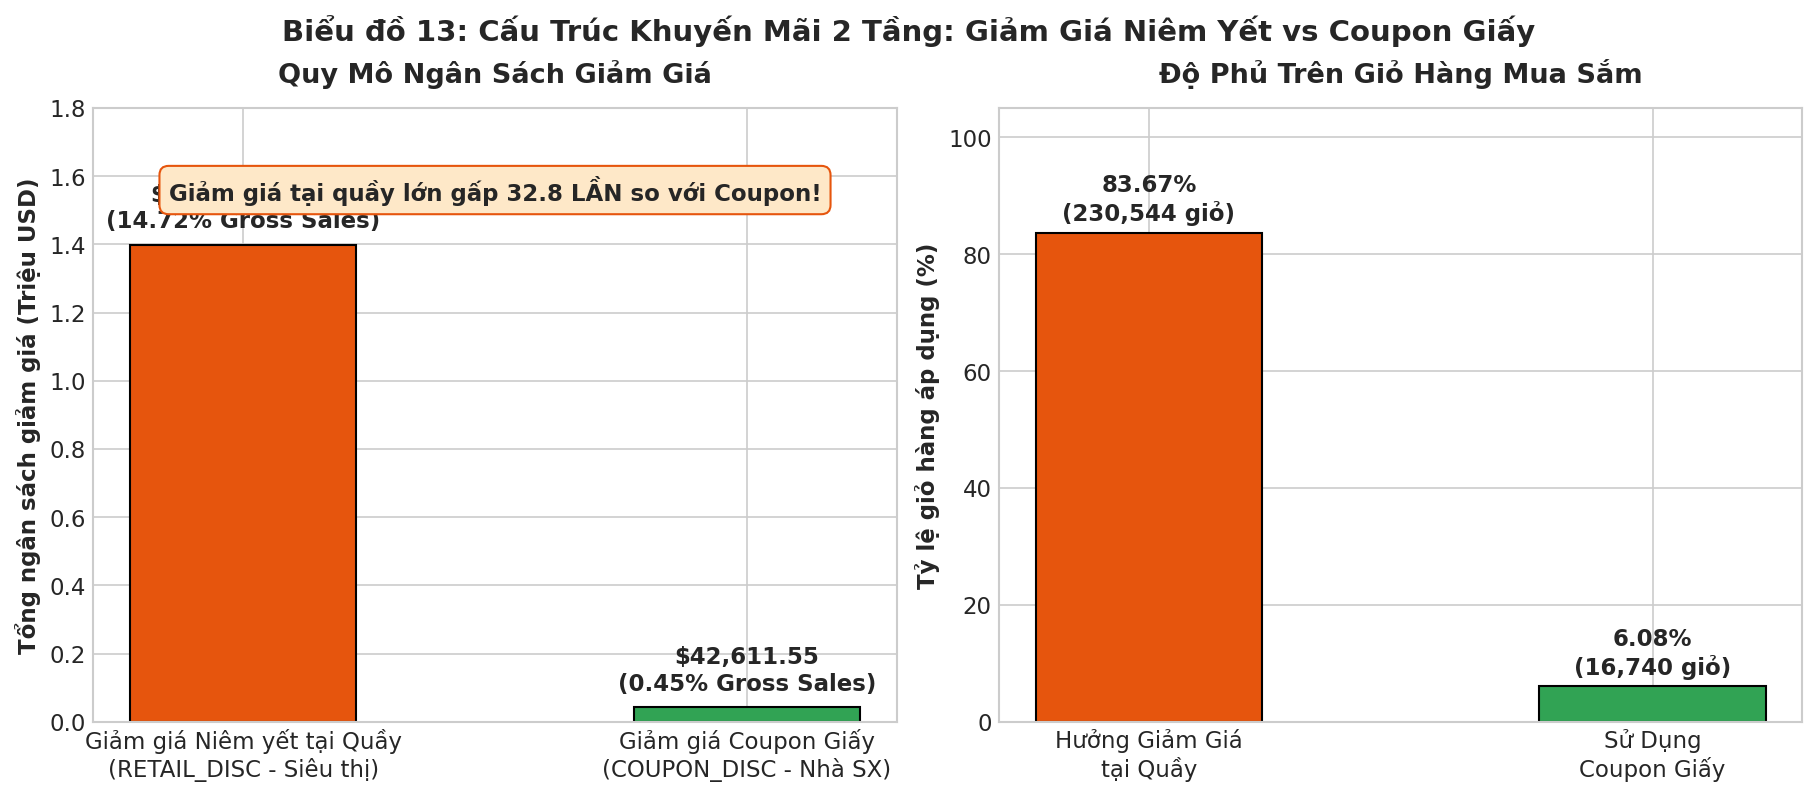
\includegraphics[width=\linewidth,height=0.65\textheight,keepaspectratio]{../reports/figures/20_markdown_vs_coupon_spend.png}
    \end{column}
    \begin{column}{0.38\textwidth}
      \small
      \textbf{Bóc Tách Dòng Tiền Chiết Khấu:}
      \begin{itemize}\setlength{\itemsep}{2pt}
        \item \textbf{Đòn bẩy 32.8 lần:} Giảm giá tại quầy (\texttt{RETAIL\_DISC} \$1.40M) lớn gấp 32.8 lần coupon (\texttt{COUPON\_DISC} \$42.6k).
        \item \textbf{Độ phủ bất cân xứng:} Giảm giá quầy xuất hiện ở 48.7\% giỏ hàng; trong khi coupon chỉ bao phủ 6.2\% giỏ săn deal.
      \end{itemize}
      \vspace{0.08cm}
      \begin{exampleblock}{Chiến Lược Biên Lợi Nhuận}
        \footnotesize
        Siêu thị chủ động hy sinh biên lợi nhuận đại trà trên kệ; coupon chỉ là công cụ nhắm trúng đích cho nhóm khách hàng chuyên biệt.
      \end{exampleblock}
    \end{column}
  \end{columns}
\end{frame}

% ==============================================================================
% SLIDE 16: CÂU CHUYỆN 15 - SỨC THÂM NHẬP NHÃN HÀNG RIÊNG
% ==============================================================================
\begin{frame}{15. Sức Thâm Nhập Vượt Trội Của Nhãn Hàng Riêng Siêu Thị}
  \begin{columns}[c]
    \begin{column}{0.60\textwidth}
      \centering
      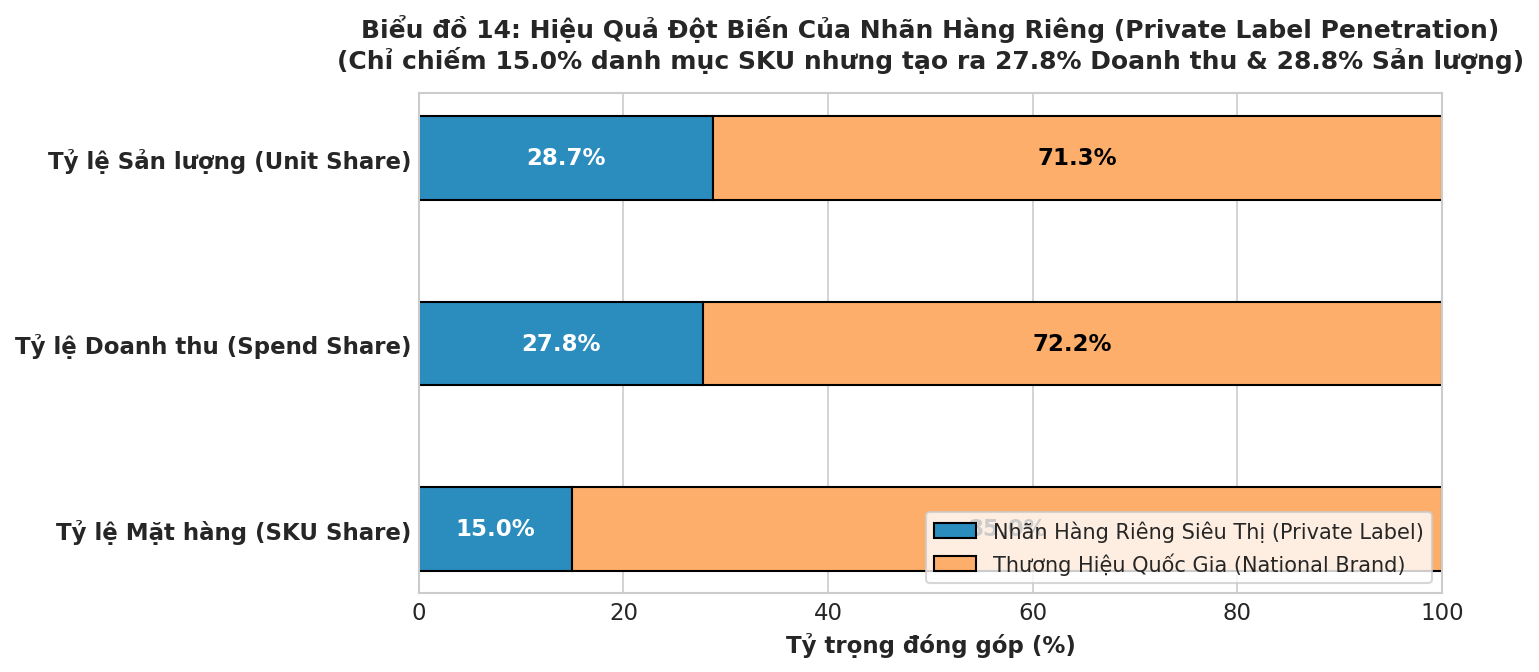
\includegraphics[width=\linewidth,height=0.65\textheight,keepaspectratio]{../reports/figures/21_private_label_penetration.png}
    \end{column}
    \begin{column}{0.38\textwidth}
      \small
      \textbf{Hiệu Quả Mặt Hàng (Private Label):}
      \begin{itemize}\setlength{\itemsep}{2pt}
        \item \textbf{Hiệu suất sinh lời 1.86x:} Chỉ chiếm 15.0\% danh mục SKU nhưng tạo ra 27.8\% doanh thu và 28.8\% sản lượng tiêu thụ.
        \item \textbf{Vượt trội thương hiệu quốc gia:} Hiệu suất trên mỗi SKU cao gấp 2.18 lần so với National Brand (0.85x).
      \end{itemize}
      \vspace{0.08cm}
      \begin{alertblock}{Chiến Lược Danh Mục Mặt Hàng}
        \footnotesize
        Nhãn riêng là lựa chọn ``chất lượng tốt - giá hợp lý'' của người tiêu dùng; vũ khí chiến lược giữ chân khách và tối ưu biên lãi gộp.
      \end{alertblock}
    \end{column}
  \end{columns}
\end{frame}

% ==============================================================================
% SLIDE 17: CÂU CHUYỆN 16 - NHỊP ĐIỆU THỜI GIAN VI MÔ
% ==============================================================================
\begin{frame}{16. Nhịp Điệu Thời Gian Vi Mô: Ngày Trong Tuần \& Khung Giờ Vàng}
  \begin{columns}[c]
    \begin{column}{0.60\textwidth}
      \centering
      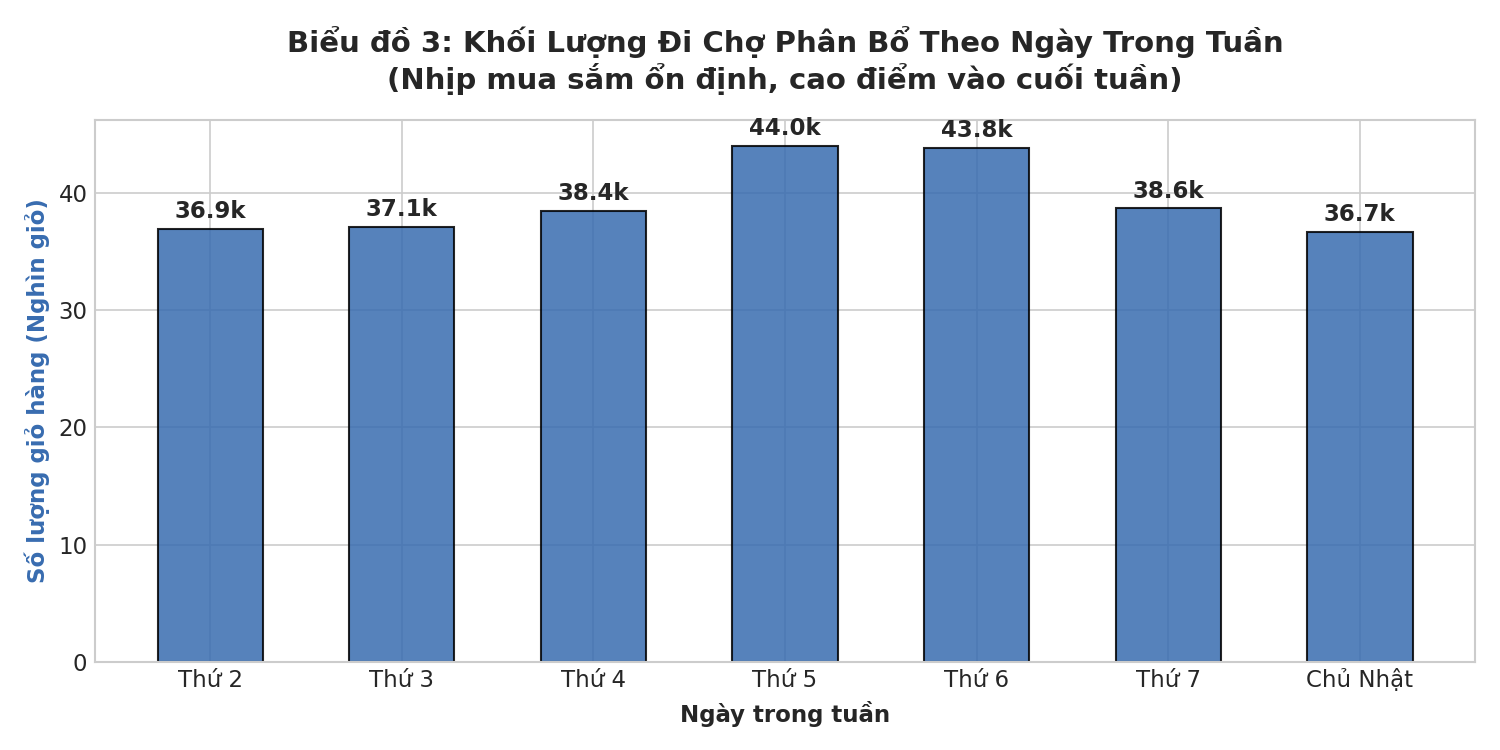
\includegraphics[width=0.48\linewidth,height=0.62\textheight,keepaspectratio]{../reports/figures/03_day_of_week_distribution.png}
      \hfill
      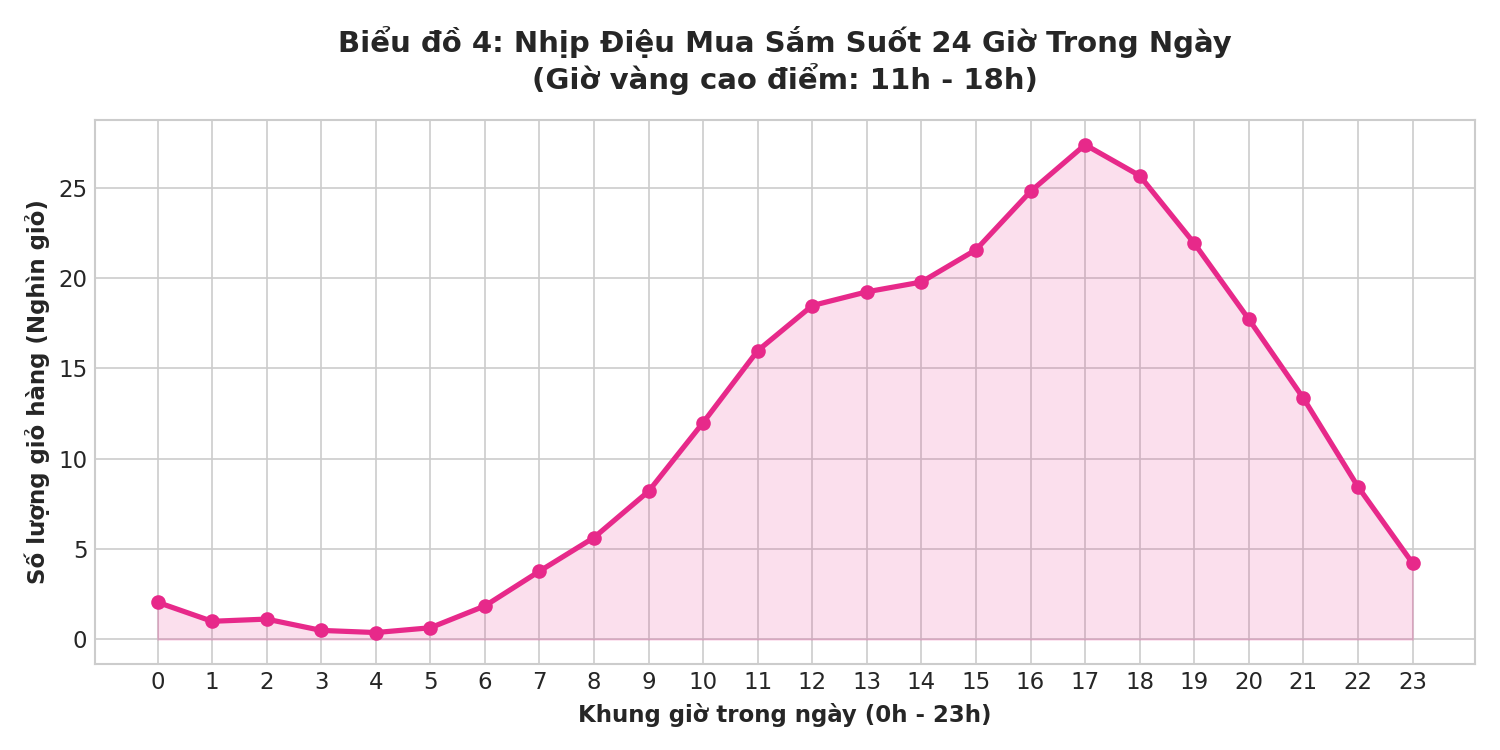
\includegraphics[width=0.48\linewidth,height=0.62\textheight,keepaspectratio]{../reports/figures/04_hourly_shopping_rhythm.png}
    \end{column}
    \begin{column}{0.38\textwidth}
      \small
      \textbf{Quy Luật Nhịp Điệu Mua Sắm:}
      \begin{itemize}\setlength{\itemsep}{2pt}
        \item \textbf{Cuối tuần tập trung (+32\%):} Thứ Bảy và Chủ Nhật chiếm gần 1/3 tổng lượng giao dịch cả tuần.
        \item \textbf{Khung giờ vàng (11h--18h):} Chiếm 65\% lưu lượng trong ngày; đạt đỉnh 14h--17h khi các hộ gia đình chuẩn bị bữa tối.
      \end{itemize}
      \vspace{0.08cm}
      \begin{exampleblock}{Vận Hành \& Lịch Trình Tiếp Thị}
        \footnotesize
        Điều phối ca trực quầy thu ngân \& nhân viên đồ tươi vào giờ cao điểm; cài đặt trigger notification CRM tự động sáng thứ Sáu.
      \end{exampleblock}
    \end{column}
  \end{columns}
\end{frame}

% ==============================================================================
% SLIDE 18: MA TRẬN ÁNH XẠ EDA SANG HỆ THỐNG ĐẶC TRƯNG HỌC MÁY & VẬN HÀNH
% ==============================================================================
\begin{frame}{17. Chuyển Hóa Phát Hiện EDA Sang Đặc Trưng ML \& Vận Hành CRM}
  \centering
  \fontsize{7pt}{8.2pt}\selectfont
  \renewcommand{\arraystretch}{0.88}
  \begin{tabularx}{\textwidth}{p{3.2cm}Y>{\raggedright\arraybackslash}p{4.6cm}}
    \toprule
    \textbf{Trụ Cột Phát Hiện} & \textbf{Căn Cứ Định Lượng (2.6M Giao Dịch)} & \textbf{Ứng Dụng Chuyển Giao: ML vs Vận Hành} \\
    \midrule
    \textbf{1. Nhịp mua \& Đồ tươi} & 92.4\% mua lại trong $\le 14$ ngày; đồ tươi kéo chu kỳ ngắn hơn 1.8 ngày & \textbf{Đặc trưng ML:} \texttt{days\_since\_last\_basket}, \texttt{urgency\_ratio}, \texttt{days\_since\_perishable} \\
    \addlinespace[1pt]
    \textbf{2. Giỏ hàng \& Mỏ neo đa ngành} & AOV P50 = \$18.1, P90 = \$63.4; mua $\ge 12$ ngành đạt 96.5\% (+64.7\%) & \textbf{Đặc trưng ML:} \texttt{spend\_30d/90d}, \texttt{aov\_90d}, \texttt{department\_breadth\_90d} \\
    \addlinespace[1pt]
    \textbf{3. Tiếp thị \& Lòng trung thành} & Dùng coupon chi tiêu gấp 2.5x; 73.4\% tiền ở shop ruột; Loại A đổi 45\% & \textbf{Đặc trưng ML:} \texttt{coupon\_redempt\_count\_180d}, \texttt{store\_loyalty\_index}, \texttt{is\_targeted\_campaign} \\
    \addlinespace[1pt]
    \textbf{4. Nhân khẩu \& Quy mô hộ} & Nhà đông con chi tiêu cao hơn +39.4\%; gán UNKNOWN cho 68\% hộ & \textbf{Đặc trưng ML:} \texttt{household\_size}, \texttt{kid\_category}, \texttt{income\_group} \\
    \addlinespace[1pt]
    \textbf{5. Phân hóa CLV \& Pareto} & Top 20\% hộ gánh 53\% tiền (Gini = 0.50); cần 44\% hộ cho 80\% tiền & \textbf{CRM VIP:} Ưu đãi giữ chân khách VIP; \textbf{ML:} Dùng \texttt{spend\_180d} chống rò rỉ \\
    \addlinespace[1pt]
    \textbf{6. Chiết khấu \& Coupon} & Markdown kệ gấp 32.8x coupon (\$1.4M vs \$42.6k); phủ 48.7\% giỏ & \textbf{Chiến Lược Giá:} Tối ưu chiết khấu niêm yết bảo toàn biên lợi nhuận ròng \\
    \addlinespace[1pt]
    \textbf{7. Nhãn riêng \& Khung giờ vàng} & Private Label tạo 27.8\% tiền (1.86x); 65\% giao dịch rơi vào 11h--18h & \textbf{Vận Hành:} Mở rộng SKU nhãn riêng; điều phối ca trực \& tin nhắn T6 \\
    \bottomrule
  \end{tabularx}
  \vspace{0.06cm}
  \centering
  \footnotesize
  \textcolor{accentOrange}{\textbf{Kỷ Luật Thời Gian:}} 100\% đặc trưng ML tính tại $DAY \le t_0$, triệt tiêu rò rỉ dữ liệu song hành cùng khuyến nghị vận hành thực chiến.
\end{frame}

% ==============================================================================
% SLIDE 19: TỔNG KẾT GIAI ĐOẠN EDA
% ==============================================================================
\begin{frame}{18. Tổng Kết Giá Trị Nền Tảng Của Giai Đoạn EDA}
  \begin{columns}[T]
    \begin{column}{0.48\textwidth}
      \textbf{4 Đóng Góp Nền Tảng Cho Dự Án:}
      \begin{enumerate}\setlength{\itemsep}{4pt}
        \item \textbf{Khung Dự Báo Khoa Học:} Dựa trên 92.4\% chu kỳ hồi tiếp thực nghiệm, xác lập cửa sổ dự báo tối ưu $\Delta t = 14$ ngày.
        \item \textbf{Chuẩn Hóa Dữ Liệu Sạch:} Loại 942 giỏ hủy/tặng 0đ, khử trùng 5,164 bản ghi coupon, bảo toàn trọn vẹn 100\% tập 2,500 hộ.
        \item \textbf{Cơ Sở Thiết Kế Đặc Trưng:} Chuyển hóa \textbf{15 phát hiện định lượng cốt lõi} thành 28 đặc trưng ML chất lượng cao cùng chiến lược vận hành.
        \item \textbf{Kiểm Định Vững Chắc:} Xác nhận tỷ lệ mục tiêu ổn định ở mức 68.25\%, không có hiện tượng trôi dạt dữ liệu theo thời gian.
      \end{enumerate}
    \end{column}
    
    \begin{column}{0.48\textwidth}
      \begin{exampleblock}{Ý Nghĩa Chuyển Giao Sang Mô Hình Hóa}
        EDA không chỉ dừng lại ở mô tả thống kê, mà đóng vai trò \textbf{la bàn toán học} định hướng:
        \begin{itemize}\setlength{\itemsep}{3pt}
          \item Chiến lược lấy mẫu trượt thời gian (Multi-cutoff temporal split).
          \item Thiết lập hàm mục tiêu và nhóm tính năng ưu tiên cao nhất.
          \item Cung cấp cơ sở nghiệp vụ vững chắc để giải thích mô hình (SHAP \& Feature Importance).
        \end{itemize}
      \end{exampleblock}
      \vspace{0.25cm}
      \centering
      \textbf{\large Xin Cảm Ơn! Lắng Nghe Câu Hỏi (Q\&A)}
    \end{column}
  \end{columns}
\end{frame}

\end{document}
